\chapter{Introduction}
\label{chapter-introduction}
\begin{ChapAbstract}
This chapter overviews e-commerce within fashion retail, focusing on the challenges associated with personalized and immersive experiences. We first discuss two significant online shopping problems, which involve virtual try-on technologies and fashion recommendation systems, and investigate various approaches to tackle those problems. Next, we describe the main contributions of this thesis to bridge the gap between physical and online fashion retail. Finally, the organizational structure of the thesis is presented, offering a concise overview of the subsequent chapters and their contents.
\end{ChapAbstract}

%%%%%%%%%%%%%%%%%%%%%%%%%%%%%%%%%%%%%%%%%%%%%%%%%%%%%%%%%%%%%%%%
\section{Overview}
Nowadays, the fashion industry has become an important part of people's lives. The development of digital globally and the recent pandemic has led to changes in consumer behaviour: e-commerce is increasingly popular and developed. Traditional retail shop owners also expand their stores on online platforms such as Amazon, Zalando, etc. Because of this, it is hardly surprising that the fashion e-commerce market will continue to flourish and diversify at an extraordinary pace. The global fashion e-commerce market is expected to reach a value of over 820 billion U.S. dollars in 2023 and could be 1.2 trillion U.S. dollars in 2027~\cite{Fashion2327-Statista2023} (details are shown in~\autoref{fig:market-forecast}). Nevertheless, the transition from traditional in-store shopping to online shopping presents distinctive challenges, such as the time-consuming process of item selection without some recommendations from the sales staff, limitations in trying on clothes before making a purchase, and risks and costs associated with product transportation.

\begin{figure}[h!]
    \centering
    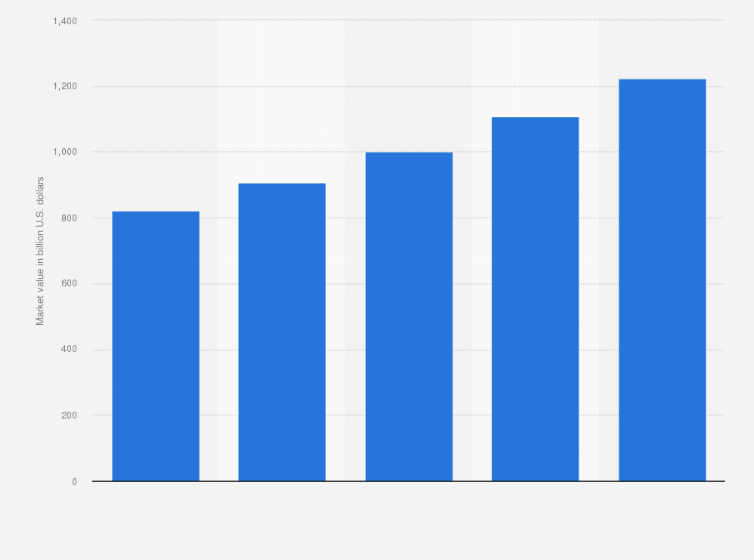
\includegraphics[width=0.7\linewidth]{content/resources/images/introduction/fashon-online-market.png}
    \caption{Fashion e-commerce market value worldwide forecast 2023-2027 (in billion U.S. dollars)~\cite{Fashion2327-Statista2023}.}
    \label{fig:market-forecast}
\end{figure}

In response to these challenges, intelligent fashion technologies have emerged as promising solutions to serve customers with the same support and comfort as in the in-person shopping experience. This thesis focuses on two significant areas of intelligent fashion: fashion recommendation systems and virtual try-on technologies. Both methodologies share a common objective of augmenting the customer experience on online platforms, thereby enabling retailers to bolster profitability. Fashion recommendation systems help users make easier and smarter shopping choices by recommending items that suit their preferences and style. Furthermore, virtual try-on technology has garnered significant attention in recent years by addressing a crucial concern of online shoppers: being concerned about how a particular in-shop garment will look when they wear it and whether it suits them. By allowing users to try on items virtually, this technology enhances the customer experience and saves the cost of damaged items for retailers. These solutions draw a new picture of online shopping and promise to take the customer experience to the next level.

%%%%%%%%%%%%%%%%%%%%%%%%%%%%%%%%%%%%%%%%%%%%%%%%%%%%%%%%%%%%%%%%
\section{Motivations}

Virtual try-on technology is a method to help customers visualize how a garment might look on their body based on an image of the person and an image of the desired item. This technology addresses a substantial challenge online shoppers encounter: having to visit a store to try on clothing items physically. According to a study of Coresight~\cite{web-try-on-motivation},  the period from March 2022 to March 2023 saw a notable 24.4\% average return rate for online clothing orders in the United States, which is equivalent to \$38 billion in returns. Moreover, 53\% of the respondents revealed that their primary reason for returns was the ill-fit of that garment during try-on (\cite{web-try-on-motivation}).

\begin{figure}[h!]
    \centering
    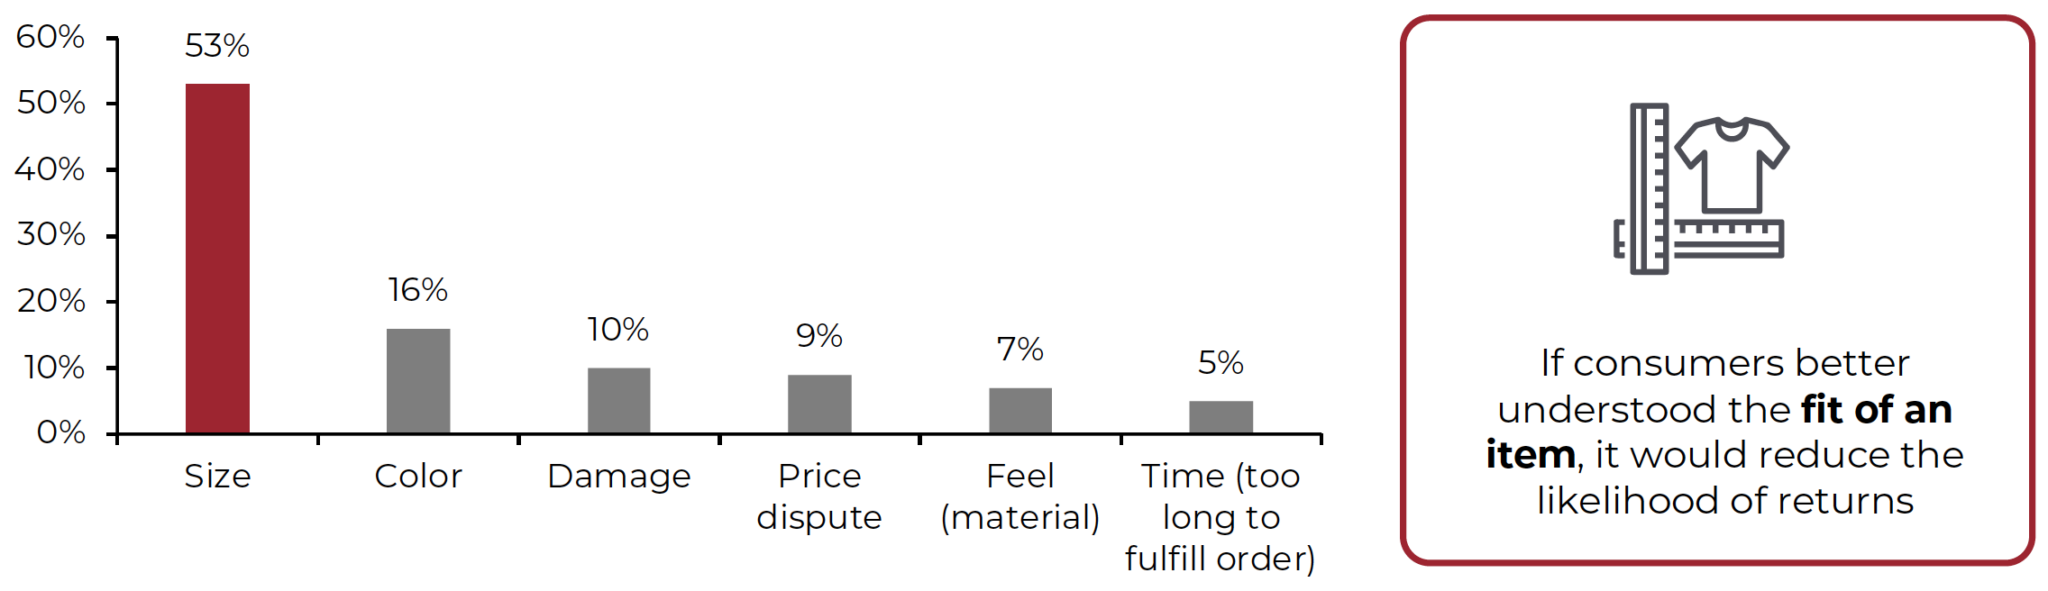
\includegraphics[width=0.7\linewidth]{content/resources/images/introduction/motivation-try-on.png}
    \caption{Reasons for garment returns from March 2022 to March 2023 (\% of Respondents)}
    \label{fig:try-on-motivation}
\end{figure}

As a result, there is a growing interest in virtual try-on, demonstrating the potential to enhance shopping experiences by integrating Augmented Reality (AR). However, existing works on image-based virtual try-on mostly do not put their concern about the complexity of their models, resulting in challenges when applying them in real-time scenarios. This motivates us to investigate the potential of a faster and more resource-efficient virtual try-on method while ensuring the fidelity of the outcomes. 

Fashion recommendation has always been crucial to modern fashion e-commerce systems due to its numerous benefits. According to a study of ViSenze~\cite{web-recommendation-motivation}, recommendations can increase conversion rates by up to 300\% and increase revenue by up to 31\%. It saves users valuable time and effort by curating multiple sets of items that align with their preferences and style. Instead of spending hours searching for fashion items online or in physical stores, users can rely on these recommendations to discover new and relevant clothes. Moreover, these recommendations help users explore a wider range of options, introducing them to different styles or brands. This encourages users to try out something they might not have considered before, thus improving the fashion industry's overall revenue. Additionally, as 71\% of consumers feel frustrated when their shopping experience is impersonal~\cite{web-recommendation-motivation}, fashion recommendation can simplify decision-making and increase user satisfaction by presenting curated options tailored to individual preferences. Ultimately, fashion recommendation has proven its usefulness by assisting users in discovering new styles, saving time, and making informed fashion choices.

%%%%%%%%%%%%%%%%%%%%%%%%%%%%%%%%%%%%%%%%%%%%%%%%%%%%%%%%%%%%%%%%
\section{Objectives and Main Contributions}
The primary objective of this thesis is to investigate and address two significant challenges in the field of fashion e-commerce: virtual try-on and fashion recommendation. By leveraging intelligent systems and cutting-edge method technologies, we aim to develop innovative solutions that enhance the online shopping experience and bridge the gap between the physical and digital realms of fashion retail.

To address the previous virtual try-on method issues, we aim to propose a framework that can achieve faster run time and less memory consumption while producing results of the same quality. Thus, it can pave the potential of integrating image-based virtual try-on into real-time AR scenarios.

Regarding the fashion recommendation problem, we focus on taking a fashion item as the reference item and recommending based on the visual features of that item. This research explores multiple approaches to produce meaningful results for such a problem. These approaches include intra-category similar item retrieval, inter-category complementary item retrieval, and text feedback-guided item retrieval. We also study incorporating approximate searching methods into these approaches to enhance the system's overall performance.

Another important objective of this thesis is to create an intelligent system for online shopping support, including web and AR applications. We aim to combine the power of fashion recommendation and virtual try-on in this system, offering new possibilities for personalized and immersive interactions between consumers and online fashion platforms.

The main contribution of this thesis can be summarized as follows:
\begin{itemize}
    \item Propose a virtual try-on framework based on knowledge distillation learning. We can achieve a lightweight network, reducing inference time and memory consumption, thus making it easier to deploy and operate on AR devices.
    \item Introduce an automatic fashion-pose data generation pipeline designed to enrich existing fashion datasets by synthesizing new person poses from a single image of that person.
    \item Investigate various ways to recommend fashion items from a reference image. These approaches include retrieving intra-category similar items, inter-category complementary items and text feedback-guided items. We also propose Outfit Retrieval Transformer to address the complementary item retrieval task.
    \item Incorporate approximate searching for retrieval, which runs significantly faster while producing nearly the same results as exhaustive methods.
    \item Build an AR application for virtual try-on, which can reduce the risk of damage to real clothes for shops.
    \item Develop a smart fashion assistant web application tailored for the fashion e-commerce industry, which integrates virtual try-on functionality and fashion recommendation capabilities, enhancing the overall user experience and increasing customer satisfaction in the fashion e-commerce sector. 
\end{itemize}


% The specific objectives of this research are as follows:


%%%%%%%%%%%%%%%%%%%%%%%%%%%%%%%%%%%%%%%%%%%%%%%%%%%%%%%%%%%%%%%%
\section{Thesis Organization}

This thesis is organized into 7 chapters: 

\textbf{Chapter 1}: This chapter overviews e-commerce within fashion retail, focusing on the challenges associated with personalized and immersive experiences. We first discuss two significant online shopping problems, which involve virtual try-on technologies and fashion recommendation systems, and investigate various approaches to tackle those problems. Next, we describe the main contributions of this thesis to bridge the gap between physical and online fashion retail. Finally, the organizational structure of the thesis is presented, offering a concise overview of the subsequent chapters and their contents.

\textbf{Chapter 2}: This chapter provides an overview of the fundamental knowledge relevant to our thesis. We present a list of Computer Vision problems that play important roles in our proposed approach.

\textbf{Chapter 3}: This chapter presents an overview of the literature in the virtual try-on and fashion recommendation fields. In the domain of virtual try-on, we introduce recent image virtual try-on approaches. Besides, some commercial products and their technology are discussed to provide a comprehensive view of this field. Moving on to fashion recommendation, we introduce related works centering on visual-based fashion recommendations. Finally, we discuss techniques for similarity search, including exhaustive and approximate methods applied to our recommendation approaches.

\textbf{Chapter 4}: In this chapter, we propose Distilled Mobile Real-time Virtual Try-On (DM-VTON), which focuses on synthesizing try-on images with increased speed compared to previous methods while ensuring accuracy. Our approach is based on a knowledge distillation scheme that leverages a strong Teacher network as supervision to guide a Student network without relying on human parsing. Notably, we introduce an efficient Mobile Generative Module within the Student network, significantly reducing the runtime while ensuring high-quality output. Additionally, we propose Virtual Try-on-guided Pose for Data Synthesis to address the limited pose variation observed in training images. Finally, we provide the experimental details of our proposed method, and then we present a comparative study of DM-VTON with state-of-the-art methods.

\textbf{Chapter 5}: In this chapter, we address the problem of recommending items given a reference fashion item. We carefully investigate three approaches to retrieving items: similar items within the same category, complementary items from other categories, and items guided by text feedback. 
In terms of retrieving intra-category similar items and text feedback-guided items, we employ a pretrained CLIP-based model and receive remarkable results. As for the inter-category complementary item retrieval, we consider it a Natural Language Process problem and propose Outfit Retrieval Transformers (ORT), which utilizes the Transformers architecture. Through experiments, ORT proves its effectiveness and can produce reasonable recommendations. Because using an embedding to query items from a dataset plays an important role in recommendation, we analyze various approximate searching methods and compare them with the exhaustive K-Nearest Neighbor algorithm regarding query time and accuracy.

\textbf{Chapter 6}: This chapter presents our applications that assist customers in e-commerce based on the methods presented, including Smart Fashion Assistant, a system for online shopping support, and Magic Mirror, an application that allows users to try on clothing items virtually in an augmented reality scenario. We present an overview of each application, followed by the details of the conducted experiments, including a pilot study to evaluate their effectiveness and user satisfaction.

\textbf{Chapter 7}: We conclude our work by summarizing the results obtained and discussing the potential for future research directions. In this thesis, we solve two major problems in online fashion shopping: virtual try-on and fashion recommendation. Through intensive experiments, we prove the applicability and efficiency of our solutions and further demonstrate them in demo applications. The feedback we gained from the pilot study shows that our work still has some limitations, which we plan to improve in future works.